\chapter{物态变化}\label{chapter-change-of-state-of-matter}

固体、液体和气体是通常存在的三种物质状态.在一定条件下,这三种物质状态可以相互转化,即发生物态变化,水结成冰或变成水蒸气就是常见的物态变化的例子.物态变化跟日常生活和工农业生产有密切关系,有许多实际应用,在初中我们学过一些物态变化的知识,这一章进一步扩大和加深这方面的知识,同时学习一些新知识.

\section{熔解和凝固}
物质从固态变成液态叫做熔解,从液态变成固态叫做\textbf{凝固}.

我们知道,固体分晶体和非晶体.晶体物质和非晶体物质在熔解和凝固时情况是不同的.晶体有一定的熔解温度——熔点.给晶体加热,当温度升高到熔点时,晶体开始熔解,在熔解过程中温度保持不变,到全部熔解后,温度才继续上升.它们的液体冷却时,温度降低到熔点时开始凝固,在凝固过程中温度也保持不变,到全部凝固后,温度才继续下降.

非晶体没有一定的熔点,温度升高时,非晶体先是由硬变软,再逐渐变成粘稠状液体,最后逐渐变成液体.在整个过程中,温度不停地上升,没有一定的熔解温度,冷却时,随着温度
的下降,液体由稀变稠,由软变硬,最后成为固体,在整个过程中,温度不停地下降,没有一定的凝固温度.

晶体物质熔解和凝固时的特点,可用晶体的微观结构来解释.在晶体中,微粒排列成有规则的空间点阵,维持这种规则排列的是微粒之间的相互作用;微粒的热运动不足以克服这种相互作用,微粒一般只能在平衡位置附近做无规则的振动.给晶体加热时,晶体从外界得到能量,微粒的热运动加剧.达到一定的温度时,一部分微粒具有了足够的动能,能够克服微粒间的作用力,离开平衡位置.这时晶体的点阵结构被破坏,晶体开始熔解,在熔解过程中,外界供给晶体的能量,全部用来破坏晶体的点阵结构,增加分子间的势能,所以温度不发生变化.凝固时,情况正好相反.微粒排列成点阵结构时,微粒间的势能减小,因此虽然放出能量,温度却保持不变,直到全部凝固成晶体.

非晶体的微观结构本来就跟液体类似,非晶体在熔解过
程中不必为破坏点阵结构而消耗能量,所以温度不停地上升.

实验表明,大多数物质熔解时体积膨胀,凝固时体积缩小.然而也有少数物质跟上述情况相反,例如水、灰铸铁、锑、铋等,它们在熔解时体积缩小,凝固时体积膨胀.用铸铁浇铸成的工件,形状跟铸模完全相似,正是利用了铸铁凝固时体积膨胀的特点.水结冰时体积膨胀,所以在冬季水管和盛水的容器常会冻裂,需要加以防止.

物质的熔点跟压强有关系,熔解时体积膨胀的物质,如果所受的压强增大,熔解将受到阻碍,只有在更高的温度下才
能熔解,所以熔点升高,熔解时体积缩小的物质,如果所受的压强增大,会促进熔解的进行,所以熔点降低.冰在熔解时体积缩小,因而冰在受到巨大的压强时,在0$^\circ$C以下也能熔解.不过压强对熔点的影响并不显著,例如,每增如1标准大气压,冰的熔点才降低0.0075$^\circ$C.

表~\ref{tab_B_5-1} 列出了几种物质在1标准大气压下的熔点.

\begin{table}[htbp]
	\centering
	\caption{}\label{tab_B_5-1}
	\begin{tabular}{cccc}
	\toprule
	物质 & 熔点($^\circ$C) & 物质 & 熔点($^\circ$C) \\
	\midrule
	氦 & $-$272 & 铅 & 327\\
	氢& $-$259 & 铝 & 660\\
	酒精& $-$117 & 银 & 962\\
	氨& $-$77.7 & 金 & 1064\\
	水银& $-$39 & 铜 & 1083\\
	冰& 0 & 铁 & 1535\\
	萘&80 & 钨 & 3410\\
	锡&232   & 碳 & 3550\\
	\bottomrule
	\end{tabular}
\end{table}

一般说来,纯物质中掺进另一种物质,熔点要降低.例如
海水比淡水的熔点低.冰和食盐的混合物,熔点可以降低到零下二十多摄氏度,冰和氯化钙的混合物,熔点可以降低到零下五十多摄氏度.

某些合金的熔点较低,例如铅锑合金的熔点为246$^\circ$C,锡铅合金的熔点为170$^\circ$C,由铋、镉、锡、铅组成的伍德合金,其熔点仅 70$^\circ$C.这些低熔点合金在生产技术中具有广泛的应用.

熔点是物质的重要性质之一,在实际中常常要根据需要选用不同熔点的物质,例如,制做白炽灯丝要用熔点高的钨,
而焊接电路则用熔点较低的铅锡合金.

\section{熔解热}
晶体在熔解过程中不断从外界吸收热量,但温度却保持不变.吸收的热景绝大部分用于破坏晶体的点阵结构,增加分子势能,对大多数熔解时体积增大的物质来说,还有一部分热量用来克服外界压强做功.不过体积变化不大,这个功很小.

质量相等的不同晶体溶解时吸收的热量是不同的.\textit{单位质量的某种物质熔解成同温度的液体时吸收的热量,叫做这种物质的熔解热}.在国际单位制中,熔解热的单位是焦/千克.

液体凝固时要放出热量.单位质量的某种物质凝固时放出的热量等于它的熔解热.显然这是符合能量守恒定律的.

物质的熔点跟压强有关系,在不同的熔解温度下,物质的熔解热也略有不同.表~\ref{tab_B_5-2} 列出了几种物质在1标准大气压下的熔解热.

\begin{table}[htbp]
	\centering
	\caption{}\label{tab_B_5-2}
    \begin{tabular}{cccc}
  \toprule
 物质 & 熔解热(${\rm J}/{\rm kg}$) & 物质 & 熔解热(${\rm J}/{\rm kg}$) \\
  \midrule
  铝 & $3.96\times 10^5$ & 萘 & $1.51\times 10^5$\\
  冰& $3.35\times 10^5$ & 锡 & $0.6\times 10^5$\\
  镍& $2.99\times 10^5$ & 铅 & $0.25\times 10^5$\\
   铁& $2.67\times 10^5$ & 水银 & $0.11\times 10^5$\\
  铜& $2.05\times 10^5$ & 二氧化碳 & $1.81\times 10^5$\\
   钨& $1.92\times 10^5$ & 金 & $0.64\times 10^5$\\
    \bottomrule
   \end{tabular}
\end{table}

熔解热常用字母$\lambda$表示.知道了熔解热,就可以算出质量为$m$的物质熔解时吸收的热量$Q$:
\[Q=\lambda m \]

熔解热可以用量热器测定.现在以冰为例来说明.在量热器中装入已知质量的水,测出水的温度,然后把正在熔解的冰块(温度为0$^\circ$C)放入量热器的水中,冰将继续熔解,水的温度下降.测出冰块全部熔解后水的末温度和的质量.根据前后两次测得的水的质量,可以求出冰块的质量,冰块熔解成水并从0$^\circ$C升高到末温度吸收的总热量,等于量热器中原来的水和小筒从初温度下降到末温度放出的热量,从这个关系就可以求出冰的熔解热.

例如,如果已知铜制量热器小筒的质量是150克,里面装着100克16$^\circ$C的水.放入9克0$^\circ$C的冰,冰完全熔解后水的温度是9$^\circ$C.利用这些数据就可以求出冰的熔解热.

9克0$^\circ$C的冰熔解为0$^\circ$C的水,再升高到9$^\circ$C,总共吸收
的热量
\[Q_{\text{吸}}=m_{\text{冰}}\lambda +m_{\text{冰}}c_{\text{水}} (9^\circ {\rm C}-0^\circ {\rm C}) \]
量热器中的水和量热器小筒从16$^\circ$C降到9$^\circ$C放出的热量
\[Q_{\text{放}}=m_{\text{水}}c_{\text{水}} (16^\circ {\rm C}-9^\circ {\rm C}) +m_{\text{筒}}c_{\text{铜}} (16^\circ {\rm C}-9^\circ {\rm C}) \]
因为$Q_{\text{吸}}=Q_{\text{放}}$,所以
\[m_{\text{冰}}\lambda +m_{\text{冰}}c_{\text{水}} (9^\circ {\rm C}-0^\circ {\rm C})=\left(m_{\text{水}}c_{\text{水}}  +m_{\text{筒}}c_{\text{铜}}\right) (16^\circ {\rm C}-9^\circ {\rm C}) \]

统一单位后,把数值代入上式[铜的比热$c_{\text{铜}}=3.9\times 10^2{\rm J}/({\rm kg}\cdot ^\circ{\rm C})$],可得
\[\lambda=3.3\times 10^5{\rm J}/{\rm kg}   \]

冰的熔解热很大,1千克0$^\circ$C的冰熔解成0$^\circ$C的水吸收的热量,相当于把1千克0$^\circ$C的水升高到80$^\circ$C需要的热量.冰的这一特点对自然界有重要的意义,它使得初冬时,一个寒冷的夜晚不会把江河湖全部封冻起来,气温也不会骤然下降;初春时,一个阳光灿烂的晴天不会使冰雪全部熔解,造成江河泛滥,气温也不会骤然升高.在日常生活中,人们利用冰熔解热大的特点来冷藏食品、冰镇饮料等.

\subsection*{练习一}

\begin{enumerate}
    \item 把玻璃放在火上加热,观察它的熔解情况,看看玻璃是不是先变软,再流动.玻璃是不是晶体?
    \item 解释下面的现象:把一块冰放在支承物上(图~\ref{fig_B_5-1}),
    将两端各挂一个重物的铁丝搭在冰块上.过一段时间后可以看到,铁丝切进冰块,但是铁丝穿过冰块的地方并没有留下切口,冰仍然是完整的一块,铁丝
    为什么能切进冰块?铁丝穿过后上面的冰为什么又成了完整的一块?如果有条件,自己做这个实验.
    \begin{figure}[htbp]
      \centering
      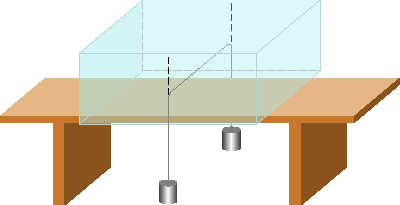
\includegraphics{fig/B/5-1.pdf}
      \caption{细铁丝穿过冰块而不留下切口}\label{fig_B_5-1}
    \end{figure}
    \item   冬季在菜窖里放上几桶水,可以使窖内的温度不致降低得很多,防止把菜冻坏.这是什么道理?如果在窖内放入200千克10$^\circ$C的水,试计算这些水结成0$^\circ$C的冰时放出的热量.这相当于燃烧多少千克干木柴所放出的热量?干木柴的
    燃烧值约为$1.26\times 10^4$千焦/千克.
\item  铜制量热器小简的质量是160克,装入200克20$^\circ$C的水.向水里放进30克0$^\circ$C的冰,冰完全熔解后水的温度是多少摄氏度?
\item  量热器的铜制小筒里盛有200克15$^\circ$C的水,小筒的质量为160克,向水里放入50克0$^\circ$C的冰,求量热器里的末温度是多少摄氏度?
\end{enumerate}


\section{蒸发}
物质从液态变成气态,叫做汽化.汽化有两种方式:蒸发和沸腾.蒸发是在液体表面进行的汽化现象.这一节我们先来研究蒸发.

我们知道,液体中的分子都在不停地运动着,它们的平均动能跟温度有关系.但在任何温度下,总有一部分分子的动能比平均动能大.那些处在液体表面层附近的动能足够大的分子,能够挣脱周围分子的引力,飞出液面,形成蒸气,这就是\textbf{蒸发},蒸气也常叫做汽.

液体温度越高,分子的平均动能就越大,具有足够大的动能因而能够飞出液面的分子也就越多.所以,温度越高,蒸发得越快.泼在地上的水夏天干得快,冬天干得慢,就是这个原因.

液体的表面积越大,处在表面层中的分子就越多,能够从液面飞出的分子也就越多.所以,表面积越大,蒸发得越快.洗过的衣服抻开晾晒比团在一起干得快,原因就在这里.

飞出液面的分子如果停留在液面附近.由于分子的热
运动,有的分子会撞到液面,被液体分子重新拉回到液体中去,这样蒸发就变慢了.如果设法把液面上形成的蒸气吹散,使汽分子不能回到液体中去,蒸发就可以加快.所以,蒸发的快慢还跟液面上气体流动的快慢有关系.气体流动得越快,蒸发得也越快,这就是吹风能够使湿东西干得快的原因.

在同样的条件下,不同液体蒸发得快慢不同.水比食油容易蒸发,汽油比水容易蒸发.容易蒸发的液体,我们常说它的挥发性大.液体的这种差别,跟它们分子间的作用力有关系.分子间作用力大的液体不容易蒸发.

在蒸发过程中,从液体中飞出的是动能较大的分子,这些分子飞出后,留在液体中的分子的平均动能必然减小,所以蒸发时液体的温度降低,这时它就要从周围的物体吸收热量,因而液体蒸发有致冷作用.穿湿衣服比穿干衣服感到冷,夏天搧扇子感到凉快,出汗后站在通风处容易着凉,都是由于蒸发致冷的缘故.蒸发致冷作用在实际中有许多应用.用火车运送容易腐烂变质的食品时,常用液态氨或液态二氧化碳的蒸发来降低车厢内的温度.在医疗中,可用液态氮迅速蒸发时的冷却作用使病灶处的细胞冷冻坏死.导弹在大气中高速飞行时,由于跟空气摩擦,会达到极高的温度.为了保护弹壳,常在弹壳表面涂上防护层,防护层的物质受热熔解和蒸发时,要
吸收大量的热量,从而降低了导弹表面的温度.

\section{饱和汽与饱和汽压}
\subsection{饱和汽} 
装在敞口容器里的液体,由于蒸发出来的汽分子能够分散到周围空间里去,所以过一段时间后液体会全部蒸发完,盛在密闭容器里的液体,即使过很长时间,也不会蒸发完,这是什么原因呢?原来在容器中的液面上同时进行着两种相反的过程:一方面分子从液面飞出来;另一方面由于液面上的汽分子不停地做无规则的热运动,有的汽分子撞到液面上又会回到液体中去(图~\ref{fig_B_5-2}).在密闭的容器中,随着液体的
不断蒸发,液面上汽的密度不断增大,回到液体中的分于数也逐渐增多,最后,当汽的密度增大到一定程度时,就会达到这样的状态:在单位时间内回到液体中的分子数等于从液面飞出去的分子数.这时汽的密度不再增大,液体也不再减少,
液体和汽之间达到了平衡状态,这种平衡叫做\textbf{动态平衡}.我们把跟液体处于动态平衡的汽叫做\textbf{饱和汽}.把没有达到饱和状态的汽叫做\textbf{未饱和汽}.在一定温度下,饱和汽的密度是一定的,未饱和汽的密度小于饱和汽的密度.

\begin{figure}[htbp]
  \centering
  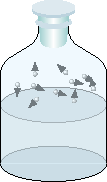
\includegraphics{fig/B/5-2.pdf}
  \caption{}\label{fig_B_5-2}
\end{figure}

饱和汽的密度随着温度而改变.温度升高时,液体分于的平均动能增大,单位时间里从液面飞出的分子数增多,原来的动态平衡被破坏,液体就继续蒸发,汽的密度继续增大,直
到达到新的动态平衡为止.所以饱汽的密度随着温度的升高而增大.温度降低时,饱和汽的密度减小.其原因请同学们自己来解释.

\subsection{饱和汽压} 

某种液体的饱和汽所具有的压强,叫做这种液体的饱和汽压.用下面的实验可以测量饱和汽压.把两根装满水银的细长玻璃管倒立在水银槽中(图~\ref{fig_B_5-3}).$a$管用作气压计.用弯曲玻璃管向$b$管中注入一些乙醚.乙醚的密度比水银小,便浮到水银面上,并在水银面上方的真空中蒸发,
同时$b$管中的水银面开始下降,当乙醚汽的密度达到饱和时,水银面上还剩有一点乙醚,$b$管中的水银面就稳定在一定的高度不再下降.$a$、$b$两管中水银面的高度差$h$就表示乙醚饱和汽压的大小.如果不用乙醚,而是向$b$管中注入水或酒精,就可以测出水或酒精的饱和汽压.
\begin{figure}[htbp]
  \centering
  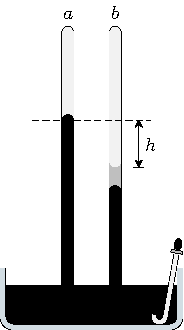
\includegraphics{fig/B/5-3.pdf}
  \caption{测量饱和汽的压强}\label{fig_B_5-3}
\end{figure}

实验表明,在相同的温度下,不同液体的饱和汽压一般是不同的.挥发性大的液体,饱和汽压大.例如,20$^\circ$C时,乙醚的饱和汽压为440毫米汞柱,水为18毫米汞柱,水银的饱和汽压很小,20$^\circ$C时仅为0.0012毫米汞柱.所以水银气压计水银柱上方的空间可以认为是真空.

\subsection{饱和汽压跟温度的关系} 

用热毛巾把图~\ref{fig_B_5-3} 中的$b$管包住,使管内的温度升高,可以看到管中的水银面下降.这表示温度升高时饱和汽压增大.如果使管内的温度降低,管中的水银面就上升,表示温度降低时饱和汽压减小.可见,\textit{饱和汽压随温度的升高而增大,随温度的降低而减小.}

饱和汽压随温度的升高而增大,这是由两方面的原因引起的,一个原因是温度升高时,饱和汽的密度增大,因此压强增大,另一个原因是温度升高时,汽分子热运动的平均速率增大,这也使得压强增大.图~\ref{fig_B_5-4} 是水的饱和汽压与温度的关系图线.从图线可以看出,温度升高时,饱和汽压增大,但是饱和汽压与温度的关系不是线性的,饱和汽压随温度的升高增大得很快.
\begin{figure}[htbp]
  \centering
  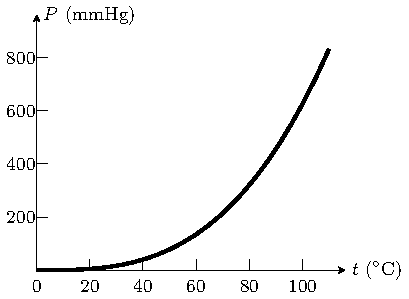
\includegraphics{fig/B/5-4.pdf}
  \caption{水的饱和汽压与温度的关系图线}\label{fig_B_5-4}
\end{figure}

饱和汽压随温度的降低而减小,其原因同学们可以自己分析一下.

\subsection{饱和汽压跟体积的关系} 

现在我们用实验来研究饱和汽
压跟体积的关系.象图~\ref{fig_B_5-5} 那样,把水银倒在一个深的容器里,再把装满水银的玻璃管倒立在这个容器中.向玻璃管里移入一些乙醚,使乙醚蒸发后水银面上还留有少量液态乙醚.这时管内乙醚的饱和汽压等于$p_0-p_k$(图~\ref{fig_B_5-5a}),其中$p_0$是大气压强.
\begin{figure}[htbp]
    \centering
    \begin{subfigure}{0.3\linewidth}
        \centering
        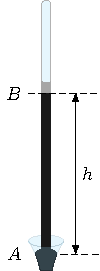
\includegraphics{fig/B/5-5a.pdf}
        \caption{}\label{fig_B_5-5a}
    \end{subfigure}
    \hfil
    \begin{subfigure}{0.3\linewidth}
        \centering
        
\includegraphics{fig/B/5-5b.pdf}
        \caption{}\label{fig_B_5-5b}
    \end{subfigure}
    \hfil
    \begin{subfigure}{0.3\linewidth}
        \centering
        
\includegraphics{fig/B/5-5c.pdf}
        \caption{}\label{fig_B_5-5c}
    \end{subfigure}
    \caption{饱和汽压跟体积无关}\label{fig_B_5-5}
\end{figure}

现在把管子往上提高一些,使水银面上乙醚汽的体积增大(图~\ref{fig_B_5-5b}),可以看到,水银面上的液态乙醚减少了,
但是管里水银柱的高度还跟原来一样.这表明,在温度不变的情况下,体积增大时饱和汽压不改变.

把提高的管子放下一些,使乙醚汽的体积减小(图~\ref{fig_B_5-5c}). 这时水银面上的液态乙醚增多,但是管中水银柱的高度仍保持不变.这表明,在温度不变的情况下,体积减小时饱和汽压也不改变.

在温度不变的情况下,饱和汽的压强不随体积而变化,可作如下的解释:当体积增大时,容器中汽的密度减小,原来的饱和汽变成了未饱和汽,于是液体继续蒸发,直到未饱和汽成为饱和汽为止;由于温度没有改变,新的饱和汽的密度跟原来的一样,汽分子热运动的平均速率也跟原来一样,所以压强不
改变.体积减小时,容器中汽的密度增大,回到液体中的分子数多于从液面飞出的分子数,于是一部分汽变成液体,直到汽的密度减小到等于该温度下饱和汽的密度为止;由于温度跟原来相同,饱和汽的密度不变,汽分子热运动的平均速率也跟原来相同,所以压强也不改变.

从上面讲的可以看出,饱和汽的压强跟体积没有关系,饱和汽的压强与温度的关系不是线性的,这些都跟理想气体的情况不同.因此,第三章所讲的理想气体定律对饱和汽是不适用的.


\subsection*{练习二}

\begin{enumerate}
\item 举出几个蒸发致冷的例子来,
\item 液面上的汽达到饱和时,还有没有液体分子从液面飞出?为什么这时从宏观上看来液体不再蒸发?
\item 饱和汽的密度怎样随温度而变化?饱和汽的压强怎祥随温度而变化?为什么这样变化?
\item 在温度不变的情况下,增大液面上饱和汽的体积时,下面的说法哪些是正确的:
\begin{enumerate}
    \item 饱和汽的质量不变,饱和汽的密度减小;
    \item 饱和汽的密度不变,饱和汽的压强也不变;
    \item 饱和汽的密度不变,饱和汽的压强增大;
    \item 饱和汽的质量增大,饱和汽的压强也增大;
    \item 饱和汽的质量增大,饱和汽的压强不变.
\end{enumerate}

\item 解释下面的现象:密闭容器中装有少量液态乙醚,当容器的温度升高时,液态乙醚逐渐减少;容器升高到一定温度
时,液态乙醚消失;容器冷却时,容器中又出现液态乙醚.
\end{enumerate}

\section{沸腾}
给液体加热,当液体升高到一定温度时,液体内部涌现出大量的气泡,升到液面破裂开,放出汽.这时整个液体发生剧烈的汽化,这种现象叫做\textbf{沸腾}.

现在我们来研究一下水的沸腾过程,给盛水的烧杯加热,原来吸附在杯底和杯壁上的空气以及溶解在水里的空气就分离出来,形成一些小气泡.由于周围的水向气泡里蒸发,所以气泡里包含的是饱和水汽和空气.杯底受热温度升高时,气泡膨胀,当体积胀大到一定程度时,气泡就脱离杯底浮起.在达到沸腾温度以前,气泡在上升过程中体积是逐渐缩小的(图~\ref{fig_B_5-6a}),这些小气泡升到液面破裂时,放出的主要是空气.
\begin{figure}[htbp]
    \centering
    \begin{subfigure}{0.4\linewidth}
        \centering
        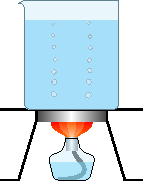
\includegraphics{fig/B/5-6a.pdf}
        \caption{}\label{fig_B_5-6a}
    \end{subfigure}
    \hfil
    \begin{subfigure}{0.4\linewidth}
        \centering
        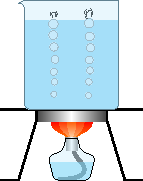
\includegraphics{fig/B/5-6b.pdf}
        \caption{}\label{fig_B_5-6b}
    \end{subfigure}
    \caption{}\label{fig_B_5-6}
\end{figure}

当杯内水的温度都升高到某一温度,气泡内的饱和汽压等于外界压强时,气泡在上升过程中体积就不再缩小.并且
由于在上升过程中周围的水还在不断向泡内蒸发,所以体积还会继续增大,直到升到液面破裂开(图~\ref{fig_B_5-6b}).这时从气泡里放出的主要是水蒸气,这时水就沸腾了.沸腾时,在液体表面和液体内部同时发生汽化,这是沸腾和蒸发的主要区别.

从上面水的沸腾过程可以看出,\textit{液体只有在它的饱和汽压等于外界压强时才能沸腾.}在外界压强是1标准大气压的情况下,水在100$^\circ$C沸腾,就是因为100$^\circ$C时水的饱和汽压为760毫米汞柱,等于外界的大气压强.

液体沸腾时的温度叫做\textbf{沸点}.外部压强改变时,液体的沸点也改变.在外部压强增大时,液体需要升到较高的温度时饱和汽压才能等于外部压强,所以沸点升高.在外部压强
减小时,液体在较低的温度下饱和汽压就能等于外部压强,所以沸点降低.上述结论可以用实验来证明.把一杯温度低于100$^\circ$C的热水放在抽气机的玻璃罩里,抽出罩里的空气,当罩里空气的压强降低到一定程度时,热水就沸腾起来(图~\ref{fig_B_5-7}).
\begin{figure}[htbp]
  \centering
  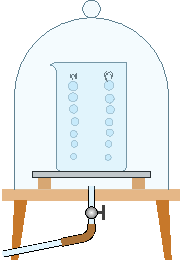
\includegraphics{fig/B/5-7.pdf}
  \caption{压强减小时水的沸点降低}\label{fig_B_5-7}
\end{figure}

离海平面越高,大气压强越小,所以高山上水的沸点较低.珠穆朗玛峰顶的气压大约只有1/3标准大气压,在那里水烧到约72$^\circ$C就沸腾了,在海拔高的山上,由于沸点低,用
普通锅煮不熟饭,需要用高压锅.高压锅内的水蒸气不容易泄出来,锅内的压强可以达到2标准大气压,锅内水的沸点接近120$^\circ$C,所以用高压锅煮饭热得快.工业上用的蒸汽锅炉也是利用增大压强来提高沸点,获得高温高压蒸汽的.如果锅炉中压强接近大气压强的10倍,水的沸点就可提高到180$^\circ$C左右.

在相同的压强下,各种物质的沸点不同.例如,在1标准大气压下,乙醚的沸点为35$^\circ$C,酒精的沸点为78$^\circ$C.利用物质的这一性质,可以对液体混合物进行分馏:给液体混合物加热,其中沸点较低的成份先蒸发出来,沸点较高的成份后蒸发出来.汽油、煤油、柴油就是在炼油厂中对石油进行分馏而得到的.

\section{汽化热}
水沸腾后,虽然继续给它加热,但是水的温度并不上升,只是有更多的水变成了水蒸气.可见,水在沸腾过程中要吸收热量.液体变为蒸气时,体积膨胀,分子间的距离增大.沸腾过程中吸收的热量,一部分用来克服分子间的引力做功增大分子势能,另一部分用于体积膨胀时克服外界压强做功.

\textit{单位质量的某种液体,变为同温度的气体时吸收的热量,叫做这种液体的汽化热.}

汽化热常用字母$L$表示.在国际单位制中,汽化热的单位是焦/千克.

不同物质的汽化热不同.表~\ref{tab_B_5-3} 列出了一些物质在1标准
大气压下沸点时的汽化热.

\begin{table}[htbp]
	\centering
	\caption{}\label{tab_B_5-3}
	\begin{tabular}{cccccc}
	\toprule
	物质  & 沸点&汽化热&  物质  & 沸点 &汽化热\\
	&($^\circ$C)&(${\rm J}/{\rm kg}$)&& ($^\circ$C)&(${\rm J}/{\rm kg}$)\\
	\midrule
	液态氦 &$-269$& $2.50\times 10^4$ &乙醚 &35& $3.52\times 10^5$\\
	液态氢&$-253$& $4.53\times 10^5$ &酒精&78& $8.55\times 10^5$\\
	液态氧&$-183$& $2.14\times 10^5$ &水&100& $2.26\times 10^6$\\
	液态二氧化碳&$-78.5$& $2.30\times 10^5$ &水银&357& $2.89\times 10^5$\\
	液态氨&$-33$& $1.37\times 10^6$ &液态铁&2750& $6.30\times 10^6$\\
	\bottomrule
	\end{tabular}
\end{table}

汽凝结为液体时要放出热量.实验表明,单位质量的汽凝结为液体时放出的热量,
等于在同一温度下液体变为相同温度的汽时的汽化热.

知道了物质的汽化热$L$,就能计算出质量为$m$的液体变为同温度的汽时吸收的
热量或质量为$m$的汽变为同温度的液体时放出的热量:
\[Q=Lm\]

在不同温度下,同一物质的汽化热不同.温度升高时,物质的汽化热变小,
这是因为温度升高时液体分子间的距离增大,液体变为汽时克服分子间的引力需
要做的功减小.

表~\ref{tab_B_5-4} 是水在不同温度下的汽化热.

\begin{table}[htbp]
	\centering
	\caption{}\label{tab_B_5-4}
	\begin{tabular}{cccc}
	\toprule
	温度($^\circ$C)&汽化热(${\rm J}/{\rm kg}$)
	&温度($^\circ$C)&汽化热(${\rm J}/{\rm kg}$)\\
	\midrule
	0& $2.50\times 10^6$ & 200 & $1.96\times 10^6$ \\
	50& $2.38\times 10^6$ & 300 & $1.38\times 10^6$ \\
	100& $2.26\times 10^6$ & 370 & $4.14\times 10^5$ \\
	\bottomrule
	\end{tabular}
\end{table}

\begin{figure}[htbp]
  \centering
  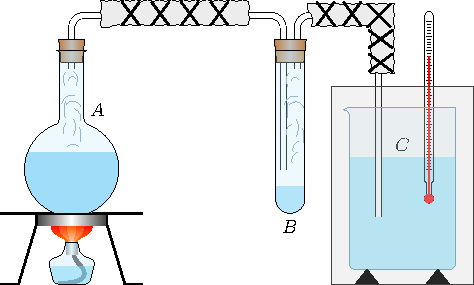
\includegraphics{fig/B/5-8.pdf}
  \caption{测定水的汽化热}\label{fig_B_5-8}
\end{figure}

水的汽化热可以用图~\ref{fig_B_5-8} 所示的实验装置来测定.用酒
精灯把烧瓶A里的水加热至沸腾.从烧瓶A里出来的蒸汽,经过试管$B$
进入装着水的量热器小筒$C$中.蒸汽经过试管$B$后,其中所含的小水滴留下来,
使得进入量热器的蒸汽中不含有水滴.蒸汽在小筒$C$中凝结时放出热量,
使小筒里的水和小筒本身的温度升高,到水温升高到相当的度数时,停止通入蒸汽.
小筒$C$的质量$m$以及其中水的质量$m_1$和温度$t_1$已在通入蒸汽前测出,
停止通入蒸汽后,再测出水的末温度$t_2$和质量$m_2$,$m_2-m_1$就是通入水中的蒸汽的质量.
水和小筒从温度$t_1$升高到$t_2$吸收的热量等于100$^\circ$C的蒸汽变为$t_2$的水放出的热量,
利用这个关系就可以求出水在100$^\circ$C时的汽化热.

\subsection*{练习三}
\begin{enumerate}
\item 在1标准大气压下,乙醚的沸点是35$^\circ$C,这个温度时乙醚的饱和汽压是多大?
\item 锡的熔点是232$^\circ$C,但是用锡焊的水壶盛着水放在1000$^\circ$C以上的火上烧,锡并不熔解.为什么?
\item 在蒸汽暖室装置的散热器里,每小时有20千克100$^\circ$C的水蒸气液化成水,
并且水的温度降低到80$^\circ$C.求散热器每小时供给房间的热量.
\item 某人在做测定水的汽化热实验时,得到的数据如下:
钢制量热器小筒的质量为200克,通入水蒸气前筒内水的质量为350克,温度为14$^\circ$C;
通入100$^\circ$C的水蒸气后水的温度为36$^\circ$C,水的质量为364克,他测得的水的汽化热是多少?
\item 容器里装有0$^\circ$C的冰和水各500克,向里面通入100$^\circ$C的水蒸气后,
容器里的水升高到了30$^\circ$C.假设容器吸收的热量很少,可以忽略不计,并且容器是绝热的,
计算一下通入的水蒸气有多少?
\end{enumerate}

\section{气体的液化}
我们知道,当饱和汽的体积减小或温度降低时,它就凝结
为液体.因此,对于未饱和汽,如果能使它变为饱和汽,就能使它液化了,怎样才能使未饱和汽变为饱和汽呢?

\subsection{把未饱和汽变为饱和汽的方法}

在一定温度下,饱和汽的密度大于未饱和汽的密度.在保持温度不变的情况下,如果用增大压强的办法来减小未饱和汽的体积,增大它的密度,那么,当密度增大到等于该温度下饱和汽的密度时,未饱和汽
就成了饱和汽.这时进一步减小汽的体积,就能使饱和汽凝结成液体.

饱和汽的密度还跟温度有关系.温度高时,饱和汽的密度大;温度低时,饱和汽的密度小.在较高温度下由于密度小而未达到饱和的未饱和汽,在保持体积不变的情况下,如果降低它的温度,那么,当温度降至未饱和汽的密度等于该温度下饱和汽的密度时,未饱和汽就成了饱和汽,这时如果继续降低温度,饱和汽就会凝结成液体.

\subsection{临界温度}

利用增大压强和降低温度的方法可以把未饱和汽变成饱和汽,从而使它变为液体.用这种方法是否能使所有的气体液化呢?

十九世纪法拉第和其他一些科学家们在这方面进行了大量的工作,他们运用增大压强和冷却的办法,把许多气体都液化了,其中有氨、氯、二氧化硫、氯化氢、硫化氢、二氧化碳等.但是,研究中发现,有几种气体,例如氧、氢、氮等,一直不能被液化,于是当时便以为这些气体是不能液化的所谓“永久气体”.

后来,进一步的研究表明,各种气体都有一个特殊的温度,在这个温度以上,无论怎样增大压强也不能使气体液化,这个温度叫做\textbf{临界温度}.氧、氢、氮等气体所以没有被液化,就是因为它们的临界温度很低,当时的低温技术尚
未获得这样低的温度.于是科学家们便努力提高低温技术,结果在二十世纪初,所有的气体都被液化了,最后一个被液化的气体是氦,它于1908年被液化,后来还被凝固成了固态.

表~\ref{tab_B_5-5} 是一些物质的临界温度.

\begin{table}[htbp]
	\centering
	\caption{}\label{tab_B_5-5}
    \begin{tabular}{cccc}
	\toprule
	  物质 &临界温度($^\circ$ C)&物质 &临界温度($^\circ$ C)\\
	\midrule
	  氦&$-268$  & 氨 & 132 \\
	氢&$-240$  & 氯 & 144 \\
	氮&$-147$  & 乙醚 & 194 \\
	氧&$-119$  & 酒精 & 243 \\
	二氧化碳&31  & 水 & 374 \\
	\bottomrule
  \end{tabular}
\end{table}

从表~\ref{tab_B_5-5} 可以看出,二氧化碳、氨、氯等气体的临界温度较高,都在室温以上,所以容易液化.而氧、氮、氢、氦的临界温度很低,所以较难液化.

液态气体有许多重要的应用.相同质量的液态气体的体积比气态小得多,便于贮存和运输,所以作为燃料的天然气常常液化后供应用户;火箭中用液态氢作燃料,用液态氧作氧化剂,液态空气蒸发时,沸点较低的氮气先蒸发,沸点较高的氧气后蒸发,因此利用液态空气可以分离出氧气和氮气.使容器中的空气液化,还可以获得压强很低的真空.

氮、氢、氦等气体的沸点很低,因此利用液态氮、氢、氦可以得到低温,低温在科学技术、医疗等方面都有重要的应用.例如,人造卫星在宇宙空间中运行时,向着太阳的一面温度很高,但是背着太阳的一面温度却很低,只有几开尔文,在这样低的温度下对卫星的材料性能有一些特殊的要求,这就要在地球上制造低温环境,进行模拟试验.低温可以治疗疾病,贮藏生物制品如血液、皮肤等,低温贮藏的细胞的活力可以保持近千年.在很低的温度下,某些物质具有特殊的性质,例如超
导电性、超流动性等,研究物质在低温下的各种性质,对认识物质的结构以及发展新技术都有重要的意义.

\section{空气的湿度}
泼在地上的水和江河湖海里的水都在蒸发,动植物的表皮和动物的呼吸也在不断地散发出水蒸气,所以我们周围的空气总含有水蒸气.一定体积的空气中含的水蒸气越多,空气就越潮湿;含的水蒸气越少,空气就越干燥.空气的干湿程度跟我们的生活和生产有密切的关系.空气太潮湿,我们会感到沉闷和窒息,东西也容易发霉;空气太干燥,我们的口腔和鼻腔会感到干燥难受,植物容易枯萎.在某些生产部门以及贮藏物品和保存名贵书画等艺术品的地方,如纺织厂、博物馆等,都要求空气保持一定的湿度.

空气的湿度可以用空气中所含水蒸气的密度,即单位体积的空气中所含水蒸气的质量来表示.由于直接测量空气中水蒸气的密度比较困难,而水蒸气的压强是随水蒸气密度的增大而增大的,所以通常都用空气中水蒸气的压强来表示空气的湿度,空气中所含水蒸气的压强叫微空气的绝对湿度.例如,空气里水蒸气的压强是15毫米汞柱,这时空气的绝对湿度就是15毫米汞柱.

空气湿度对蒸发的快慢、植物的枯萎、动物的感觉的影响不是由空气的绝对湿度来决定,而是跟空气中的水蒸气离饱和状态的远近有关系.由于饱和水蒸气的压强随温度的升高而增大,所以在空气的绝对湿度一定的情况下,气温高时,水蒸气离饱和状态远;气温低时,水蒸气离饱和状态近.例如空气
的绝对湿度是9毫米汞柱,在气温是20$^\circ$C时,水燕气离饱和状态较远(20$^\circ$C时水的饱和汽压是17.5毫米汞柱),我们就感到空气比较干燥;在气温是10$^\circ$C时,水蒸气接近饱和(10$^\circ$C时水的饱和汽压是9.2毫米汞柱),我们就感到空气很潮湿.为了表示空气中水蒸气离饱和状态的远近,物理学中引入了相对湿度的概念.

某温度时空气的绝对湿度跟同一温度下水的饱和汽压的百分比,叫做这时空气的\textbf{相对湿度}.

如果气温为20$^\circ$C时绝对湿度$p=9$毫米汞柱,因为20$^\circ$C时水的饱和汽压$P=17.5$毫米汞柱,所以这时空气的相对湿度
\[B=\frac{9}{17.5}\times 100\%=51\% \]
用公式来表示就是
\[B=\frac{p}{P}\times 100\% \]

不同温度下水的饱和汽压可以从表~\ref{tab_B_5-6} 得到.这样,知道了空气的绝对湿度,利用上面的公式就可以求出空气的相对湿度.反过来,如果知道了某一温度下的相对湿度,也可以算出绝对湿度.

在绝对湿度一定的情况下,气温降低时,相对湿度将增大.因此,在夏季有时感到白天比较干燥,夜晚比较湿润.

在住人的房间里,相对湿度为60—70\%比较适宜.

\begin{table}[htbp]
    \centering
    \caption{不同温度下水的饱和汽压(单位:毫米汞柱)}\label{tab_B_5-6}
    \begin{tabular}{cc|cc|cc|cc|cc|cc}
	\toprule
	    $t$ & $P$ &$t$ & $P$ &$t$ & $P$ &$t$ & $P$ &$t$ & $P$ &$t$ & $P$ \\
	($^\circ$C)&&($^\circ$C)&&($^\circ$C)&&($^\circ$C)&&($^\circ$C)&&($^\circ$C)\\
	\midrule
	$-$15  &  1.44  &  $-$3  &  3.67  &  9  &  8.61  &  21  &  18.65  &  33  &  37.73  &  45  &  71.88\\
	$-$14  &  1.56  &  $-$2  &  3.96  &  10  &  9.21  &  22  &  19.83  &  34  &  39.9  &  50  &  92.51\\
	$-$13  &  1.69  &  $-$1  &  4.26  &  11  &  9.84  &  23  &  21.07  &  35  &  42.18  &  60  &  149.38\\
	$-$12  &  1.83  &  0  &  4.58  &  12  &  10.52  &  24  &  22.38  &  36  &  44.56  &  70  &  233.7\\
	$-$11  &  1.99  &  1  &  4.93  &  13  &  11.23  &  25  &  23.76  &  37  &  47.07  &  80  &  355.1\\
	$-$10  &  2.15  &  2  &  5.29  &  14  &  11.9  &  26  &  25.21  &  38  &  49.7  &  90  &  525.8\\
	$-$9  &  2.33  &  3  &  5.69  &  15  &  12.79  &  27  &  26.74  &  39  &  52.44  &  100  &  760\\
	$-$8  &  2.51  &  4  &  6.1  &  16  &  13.63  &  28  &  28.35  &  40  &  55.82  &  150  &  3570.5\\
	$-$7  &  2.72  &  5  &  6.54  &  17  &  14.53  &  29  &  30.04  &  41  &  58.34  &  200  &  11659.2\\
	$-$6  &  2.93  &  6  &  7.01  &  18  &  15.48  &  30  &  31.82  &  42  &  61.5  &  250  &  29817.8\\
	$-$5  &  3.16  &  7  &  7.51  &  19  &  16.48  &  31  &  33.7  &  43  &  64.8  &  300  &  64432.8\\
	$-$4  &  3.41  &  8  &  8.05  &  20  &  17.54  &  32  &  35.66  &  44  &  68.26  &  350  &  124001.6\\
	\bottomrule
    \end{tabular}
\end{table}

\subsection*{练习四}

\begin{enumerate}
\item 说明使未饱和汽变为饱和汽的方法和道理.
\item 潮温的天气里,湿衣服不容易干,为什么?
\item 在绝对湿度相同的情况下,冬天和夏天的相对湿度哪个大?为什么?
\item 空气的绝对湿度是9毫米汞柱,气温是16$^\circ$C,相对湿度是多少?
\item 教室里空气的相对湿度是60\%,温度是18$^\circ$C,绝对温度是多少?
\end{enumerate}

\section{露点~~湿度计}
\subsection{露点} 
空气里的未饱和水蒸气,当气温逐渐降低时将逐
渐接近饱和,当气温降低到某一温度时,水蒸气达到饱和状态,这时将有水蒸气凝结成水,在物体表面上形成一层细小的露滴.

\textbf{使空气里的水蒸气刚好达到饱和时的温度,称为露点.}

空气中含的水蒸气多,气温只要少许降低一点,就达到露点,水蒸气就达到饱和;反之,空气中含的水蒸气少,气温要降低较多,才能达到露点,水蒸气才达到饱和,因此,根据露点和气温的差值,可以大致判断出空气中水蒸气的饱和程度,从而判断出相对湿度的大小.
\begin{figure}[htbp]
  \centering
  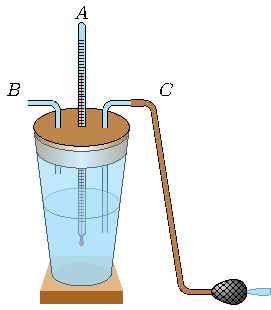
\includegraphics{fig/B/5-9.pdf}
  \caption{测定露点}\label{fig_B_5-9}
\end{figure}

露点可以用图~\ref{fig_B_5-9} 所示的装置来测定.玻璃杯里装入乙醚,杯盖上有三个孔,分别插入温度计$A$和两根弯曲的玻璃管$B$、$C$.管$C$的一端插在乙醚中,另一端连接打气球.管$B$是出气用的.用打气球向乙醚里打气,乙醚就迅速蒸发,使杯子和周围空气的湿度降低,当降低到某一温度时,杯子周围空气中的水蒸气达到饱和,杯壁上就出现一层露滴,这时温度计指示的湿度就是露点,在这个装置中如果用表面光亮的金属
杯代替玻璃杯,更容易观察到露滴的出现,效果会更好.

测出了露点,从水的饱和汽压表中查出露点时的饱和汽压,这个饱和汽压就是空气在原来温度时的绝对湿度,知道了绝对湿度,再查出原来温度下的饱和汽压,就可以求出相对湿度.

\subsection{湿度计} 
既然测出露点就能求出空气的绝对湿度和相对湿度,所以测定露点的仪器就是一种湿度计.这种湿度计叫做\textbf{露点湿度计}.

\begin{figure}[htbp]
  \centering
  \begin{minipage}[t]{0.48\textwidth}
    \centering
    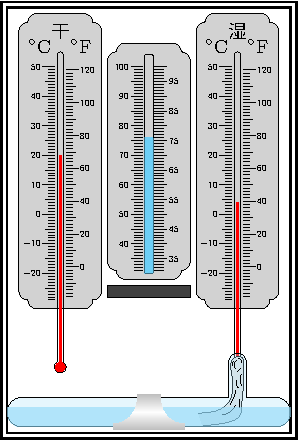
\includegraphics{fig/B/5-10.pdf}
    \caption{干湿泡湿度计}\label{fig_B_5-10}
  \end{minipage}
  \hfil
  \begin{minipage}[t]{0.48\textwidth}
    \centering
    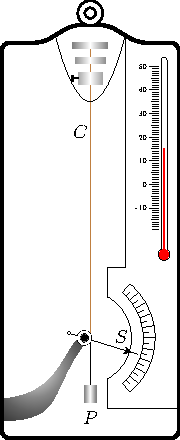
\includegraphics{fig/B/5-11.pdf}
    \caption{毛发湿度计}\label{fig_B_5-11}
  \end{minipage}
\end{figure}

还有两种常用的湿度计,一种叫做\textbf{干湿泡湿度计}(图~\ref{fig_B_5-10}).它由两支完全相同的湿度计组成,湿度计$A$叫做干泡
湿度计,用来测量空气的湿度;湿度计$B$叫做湿泡湿度计,它的水银泡上包着棉纱,棉纱的下端浸在水中,由于水的蒸发,湿度计$B$指示的湿度总是低于$A$的.$A$、$B$的湿度差叫做干湿泡湿度差,空气的相对湿度越小,即空气越干燥,湿泡湿度计$B$上的水蒸发得越快,$B$的湿度就降得越低,两支湿度计的湿度差就越大;反之,空气的相对湿度越大,即空气越潮湿,湿度计$B$上的水蒸发得就越慢,$A$、$B$的湿度差就越小.所以,干湿泡湿度差的大小跟空气的相对湿度有直接关系,如果把不同湿度时相应于不同的干湿泡湿度差的相对湿度计算出来,绘制成表或画成曲线,那么根据干湿泡湿度计上$A$、$B$两支湿度计的读数,从表或曲线上很快就可以得出空气的相对湿度.

另一种常用的湿度计叫做\textbf{毛发湿度计}(图~\ref{fig_B_5-11}).它是利用人的头发在脱脂以后,其长度会随着空气的相对湿度而变化制成的.毛发湿度计由一根或一束脱脂的毛发、指针和刻度盘组成.空气的相对湿度增大时,毛发伸长;相对湿度减小时,毛发缩短.毛发长度的变化控制指针的偏转,从刻度盘上就可以直接读出相对湿度.

三种湿度计各有不同的优缺点.露点湿度计测量准确,但是结构比较复杂,测出露点后要进行查表、计算等,使用起来不太方便.干湿泡湿度计使用比较方便,也比较准确,所以生活中大都使用这种湿度计.毛发湿度计结构简单,不易损坏,可以直接读数,还可以和自动记录装置联合使用,缺点是不太准确,要经常进行校准.

\subsection*{练习五}

\begin{enumerate}
\item 在北方,冬天戴着眼镜从寒冷的室外进入温暖的空内时,镜片上常出现一层细小的露滴.这是为什么?
\item 白天空气的绝对湿度是13.7毫米汞柱.天气预报夜里的最低温度是14$^\circ$C,如果空气的绝对湿度保持不变,夜里会不会出现露水?
\item 如果干湿泡湿度计上两支温度计的指示数字相同,这时空气的相对湿度是多少?
\item 空气的温度是20$^\circ$C,露点是12$^\circ$C,这时的绝对湿度和相对湿度是多少?
\item 空气的温度是25$^\circ$C,相对湿度是50\%,气温降低到多少摄氏度时,才会有露出现?
\end{enumerate}

\section*{阅读材料:过热液体、过冷液体和过饱和汽}
\subsection*{过热液体} 

从液体沸腾现象知道,吸附在容器壁上的空气和溶解在液体中的空气对沸腾起着重要的作用.这些空气在液体被加热时形成气泡,使得周围的液体能够向里面蒸发,成为液体内部的汽化核.在液体沸腾,气泡上升到液面破裂时,空气被放出,这样液体中的空气便越来越少,经过多次煮沸的液体,由于里面的空气已经放尽,所以加热到沸点以上也不沸腾,这种液体叫做过热液体.过热液体是不稳定的,如果有尘屑进入,或由于液体分子的运动,液体内部自发地产生极小的气泡,周围的高温液体就会迅速地向气泡内蒸发,使液
体突然剧烈地沸腾起来,发生暴沸.暴沸时甚至会使容器爆炸.为了避免这种情况,锅炉中的水在加热前应加进一些溶有空气的新水,或放进一些吸附有空气的无釉陶瓷碎块,在高能物理研究中常应用过热液体来探测高能粒子的运动径迹,使容器中的透明液体(例如液体氦、氢、丙烷、戊烷等)处于过热状态,当带电粒子通过液体时,就发生沸腾,结果在粒子经过的地方产生大量气泡,从而显示出粒子的径迹.这种仪器叫做气泡室.

\subsection*{过冷液体} 
液体凝固为晶体,需要有晶核存在.液体中的尘埃、杂质等微粒都可以作为晶核,纯净的液体由于没有晶核,在温度降低到凝固点以下时也不会凝固,这种液体叫做过冷液体.过冷液体是不稳定的,如果有尘屑进入,就立即开始凝固.

在0$^\circ$C以下的云雾中,常有一些过冷水滴.飞机在过冷水滴组成的云层中飞行时,由于机翼、机身等与水滴相碰撞,就会在这些部位结成冰层,因而增加飞机的重量,甚至使某些部位的机械操纵失灵.因此,需要采取措施防止结冰.

\subsection*{过饱和汽} 
在通常情况下,当温度降低到使未饱和汽变为饱和汽时,蒸气就凝结为液体.这是因为一般蒸气中都含有尘埃和杂质,成为蒸气凝结的凝结核,对于纯净的蒸气,即使温度降低到使它超过饱和的程度,蒸气也不凝结为液体.这种超过饱和汽密度而仍不液化的蒸气,叫做过饱和汽.过饱和汽也是不稳定的,如果其中有凝结核出现,就会发生凝结,使蒸气回到饱和状态.在原子核物理研究中观测微观粒子径迹的仪器“威尔逊云室”就利用了过饱和汽.这种仪器我们将
在高中物理第三册原子核一章中讲到.


\section*{复习题}
\begin{enumerate}
    \item 晶体和非晶体在熔解和凝固时有什么不同?怎样从它们的微观结构来说明这种不同?
    \item 什么是物质的熔解热?
    \item 什么是蒸发?怎样用分子运动论的观点来解释影响蒸发快慢的各种因素?蒸发为什么能致冷?
    \item 什么是沸腾?液体沸腾的条件是什么?为什么外界压强增大时沸点升高,压强减小时沸点降低?
    \item 什么是物质的汽化热?
    \item 什么叫饱和汽?什么叫未饱和汽?饱和汽的密度和压强跟温度有什么关系?跟体积有什么关系?怎样解释这种关系?
    \item 怎样才能使气体液化?什么叫做气体的临界温度?
    \item 什么叫做空气的绝对湿度和相对湿度?在绝时湿度保持不变的情况下,气温不同时相对湿度是否相同?为什么?
    \item 什么叫做露点?测出露点,怎样求出空气的绝对湿度和相对湿度?
    \item 干湿泡湿度计和毛发湿度计各是利用什么现象制做的?
\end{enumerate}


